\documentclass[tikz,border=4pt]{standalone}
\usepackage{libertine}
\usetikzlibrary{arrows.meta,calc,positioning,fit,backgrounds,shapes.geometric}
\definecolor{paperink}{HTML}{263441}
\definecolor{papermuted}{HTML}{647481}
\definecolor{paperline}{HTML}{CCD5DB}
\definecolor{paperblue}{HTML}{2D5F91}
\definecolor{paperbluefill}{HTML}{EFF5FA}
\definecolor{paperorange}{HTML}{B66731}
\definecolor{paperorangefill}{HTML}{FCF4EB}
\definecolor{papergreen}{HTML}{3F7558}
\definecolor{papergreenfill}{HTML}{EFF6F1}
\tikzset{
  papertext/.style={font=\footnotesize, text=paperink},
  papermini/.style={font=\scriptsize, text=papermuted},
  paneltitle/.style={font=\footnotesize\bfseries, text=paperink},
  bluebox/.style={draw=paperblue, fill=paperbluefill, rounded corners=1pt,
    line width=.6pt, font=\footnotesize, text=paperink, align=center,
    inner xsep=6pt, inner ysep=5pt},
  orangebox/.style={draw=paperorange, fill=paperorangefill, rounded corners=1pt,
    line width=.6pt, font=\footnotesize, text=paperink, align=center,
    inner xsep=6pt, inner ysep=5pt},
  greenbox/.style={draw=papergreen, fill=papergreenfill, rounded corners=1pt,
    line width=.6pt, font=\footnotesize, text=paperink, align=center,
    inner xsep=6pt, inner ysep=5pt},
  graybox/.style={draw=paperline, fill=white, rounded corners=1pt,
    line width=.6pt, font=\footnotesize, text=paperink, align=center,
    inner xsep=6pt, inner ysep=5pt},
  orangeflow/.style={-{Stealth[length=2mm]}, draw=paperorange, line width=1pt},
  blueflow/.style={-{Stealth[length=2mm]}, draw=paperblue, line width=1.15pt},
  greenflow/.style={-{Stealth[length=2mm]}, draw=papergreen, line width=1pt},
  grayflow/.style={-{Stealth[length=1.8mm]}, draw=papermuted, line width=.65pt}
}

\begin{document}
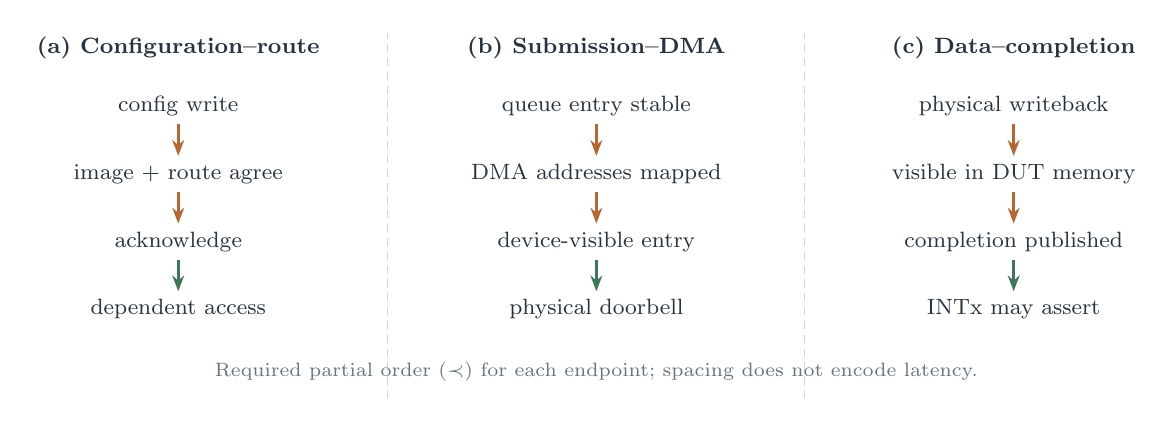
\begin{tikzpicture}[x=1cm,y=1cm]
  % Three per-endpoint happens-before chains. No global ordering is asserted.
  \foreach \x in {5.32,10.61} {
    \draw[paperline, densely dashed] (\x,.24) -- (\x,4.88);
  }
  \node[paneltitle] at (2.66,4.69) {(a) Configuration--route};
  \node[paneltitle] at (7.97,4.69) {(b) Submission--DMA};
  \node[paneltitle] at (13.27,4.69) {(c) Data--completion};

  \foreach \x/\a/\b/\c/\d in {
    2.66/{config write}/{image + route agree}/{acknowledge}/{dependent access},
    7.97/{queue entry stable}/{DMA addresses mapped}/{device-visible entry}/{physical doorbell},
    13.27/{physical writeback}/{visible in DUT memory}/{completion published}/{INTx may assert}
  } {
    \node[papertext] at (\x,3.95) {\a};
    \node[papertext] at (\x,3.09) {\b};
    \node[papertext] at (\x,2.23) {\c};
    \node[papertext] at (\x,1.37) {\d};
    \draw[orangeflow] (\x,3.72) -- (\x,3.32);
    \draw[orangeflow] (\x,2.86) -- (\x,2.46);
    \draw[greenflow] (\x,2.00) -- (\x,1.60);
  }
  \node[papermini] at (7.97,.58)
    {Required partial order ($\prec$) for each endpoint; spacing does not encode latency.};
\end{tikzpicture}
\end{document}
